\documentclass[12pt,a4paper]{extarticle}
\usepackage{graphicx}
\usepackage{titlesec}

% Font & cyrillic glyphs
\usepackage[english,russian]{babel}
\usepackage{fontspec}
\setmainfont{Times New Roman}
\setmonofont{Courier New}

% Margins
\usepackage[
    top=10mm,
    bottom=20mm,
    left=10mm,
    right=10mm
]{geometry}

% \usepackage{multicol}
\usepackage{tabularx}
\newcolumntype{H}{>{\hsize=.5\hsize}X}
\newcolumntype{S}{>{\hsize=.25\hsize}X}
\newcolumntype{s}{>{\centering\arraybackslash}S}
\newcolumntype{h}{>{\centering\arraybackslash}H}
\newcolumntype{t}{>{\ttfamily}H}

\usepackage{xltabular}
\usepackage{multirow}

\usepackage{setspace}
\setlength{\parindent}{0mm}  % Paragraph indent
\setstretch{1}  % Line height

\titleformat{\section}[hang]{\normalfont\bfseries}{\thesection}{1em}{}
\titlespacing{\section}{0pt}{4pt}{0pt}
\titleformat{\subsection}[hang]{\normalfont}{\thesubsection}{1em}{}
\titlespacing{\subsection}{0pt}{4pt}{0pt}
\titleformat{\subsubsection}[hang]{\normalfont}{\thesubsubsection}{1em}{}
\titlespacing{\subsubsection}{0pt}{4pt}{0pt}


\addto\captionsrussian{\renewcommand*\contentsname{ОГЛАВЛЕНИЕ}}

\begin{document}

\begin{titlepage}
    \begin{center}
        {\bfseries\large
        МИНОБРНАУКИ РОССИИ\par
        САНКТ-ПЕТЕРБУРГСКИЙ ГОСУДАРСТВЕННЫЙ\par
        ЭЛЕКТРОТЕХНИЧЕСКИЙ УНИВЕРСИТЕТ\par
        <<ЛЭТИ>> ИМ. В.И. УЛЬЯНОВА (ЛЕНИНА)\par
        Кафедра САПР
        
        \vspace{0.23\textheight}
        
        ОТЧЁТ\par
        по лабораторной работе №1\par
        по дисциплине <<Программирование>>\par
        Тема: Маркированная строка. Часть 1.
        
        \vspace{0.28\textheight}
        }
        \begin{table}[h!]
            \centering\large
            \begin{tabularx}{\textwidth}{p{60mm}X>{\centering\arraybackslash}p{45mm}}
                Студент гр. 4352 & \_\_\_\_\_\_\_\_\_\_\_\_\_\_\_\_\_\_\_\_ & {Даричев Е. М.} \\ [5.4mm]  % Line height
                Преподаватель    & \_\_\_\_\_\_\_\_\_\_\_\_\_\_\_\_\_\_\_\_ & {Копец Е. Е.} \\ [5.4mm]
            \end{tabularx}
        \end{table}

        \vspace{0.1\textheight}
        \large
        Санкт-Петербург\par
        2025
    \end{center}
\end{titlepage}
\setcounter{page}{2}
\tableofcontents
\newpage

% document %
\section{Исходная формулировка задания}
Преобразовать заданную строку следующим образом:
каждую точку заменить многоточием. Реализовать два варианта
задания строк: с помощью разделителей и по количеству запрашиваемых
символов.

\section{Определение неясностей}
Разделитель определяет конец строки, сохраняемой в памяти.
Маркер конца строки обозначает конец интересующей строки,
текст после маркера не влияет на результирующую строку. В
качестве этих символов могут выступать любые символы 
таблицы ASCII.

При использовании динамического выделения памяти второй вариант
ввода сводится к тому, что количество запрашиваемых символов всегда
равно длине строки. В таком случае для обработки будет забираться вся
строка.

\section{Контрольный пример}
Ниже приведены контрольные примеры, в которых в качестве разделителя принят
символ <<*>>, а в качестве маркера --- <<@>>.
\begin{table}[h]
    \centering
    \begin{tabularx}{\textwidth}{|t|t|}
        \hline
        \multicolumn{1}{|h|}{Ввод} & \multicolumn{1}{h|}{Вывод} \\ \hline
        Строка с точками. И ограничит*елем & Строка с точками... И ограничит@ \\ \hline
        Много..точек...подряд & Много......точек.........подряд@ \\ \hline
        Несколько ограничителей*** & Несколько ограничителей@ \\ \hline
        Маркер.перед.огр@аничителем* & Маркер...перед...огр@ \\ \hline
        Др!!угие."сим"волы\$\$\#*??* & Др!!угие..."сим"волы\$\$\#@ \\ \hline
    \end{tabularx}
\end{table}

\section{Ограничения, обусловленные вычислительным устройством}
Ограничения могут накладываться на максимальное количество памяти,
которое можно выделить для динамического массива символов.

\section{Организация интерфейса пользователя}
Интерфейс реализован шаблонами:

O1 (приветственное сообщение и запрос версии ввода):\\
{\ttfamily\footnotesize
Задание: Преобразовать заданную строку следующим образом: каждую точку

заменить многоточием

Даричев Егор а.г. 4352

Введите номер варианта ввода: [I1]
}

I1 (запрос версии файла): {\ttfamily\footnotesize \{1|2\}}

O2/3: {\ttfamily\footnotesize Не удалось открыть файл ввода/вывода}

O4: {\ttfamily\footnotesize Неверный номер варианта}

O5: {\ttfamily\footnotesize Вывод результата в консоль и выходной файл:\par
[формат выходного файла]}

\section{Формат файлов}
Входные и выходные файлы должны иметь следующие форматы:

\begin{xltabular}{\textwidth}{|t|t|}
    \hline
    \multicolumn{2}{|>{\centering\arraybackslash}X|}{Входные файлы} \\ \hline
    \multicolumn{1}{|h|}{Вариант 1} & \multicolumn{1}{h|}{Вариант 2} \\ \hline
    RM \normalfont //символы разделителя и маркера\par\ttfamily
    [c...]\{R|M|\}[c...] \normalfont //первая строка\par\ttfamily
    [c...]\{R|M|\}[c...] \normalfont //вторая строка\par\ttfamily
    ... &
    M \normalfont //символ маркера\par\ttfamily
    [c...]\{M|\}[c...] \normalfont //первая строка\par\ttfamily
    [c...]\{M|\}[c...] \normalfont //вторая строка\par\ttfamily
    ... \\ \hline

    \multicolumn{2}{|>{\centering\arraybackslash}X|}{Выходные файлы} \\ \hline
    \multicolumn{2}{|t|}{
    [c...]M \normalfont //первая строка\par\ttfamily
    [c...]M \normalfont //вторая строка\par\ttfamily
    ...
    } \\ \hline
\end{xltabular}

\section{Реализация ввода/вывода}
\begin{xltabular}{\textwidth}{|h|s|s|}
    \hline
    \multicolumn{1}{|h|}{Библиотека} &
    \multicolumn{1}{s|}{Ввод} &
    \multicolumn{1}{s|}{Вывод}\\ \hline
    iostream & cin > > & cout < < \\ \hline
\end{xltabular}

\section{Внутреннее представление данных}
\begin{xltabular}{\textwidth}{|
>{\hsize=.2\hsize\centering\arraybackslash\ttfamily\bfseries}X|
>{\hsize=.1\hsize\centering\arraybackslash\itshape}X|
>{\hsize=.7\hsize\centering\arraybackslash}X|
}
\hline
\multicolumn{1}{|>{\hsize=.2\hsize\centering\arraybackslash}X}{Имя переменной} &
\multicolumn{1}{|>{\hsize=.1\hsize\centering\arraybackslash}X}{Тип} &
\multicolumn{1}{|>{\hsize=.7\hsize\centering\arraybackslash}X|}{Описание} \\ \hline
ifstream & in & Входной файл \\ \hline
ofstream & out & Выходной файл \\ \hline
strings & str* & Массив считанных строк \\ \hline    
\end{xltabular}
Структура {\ttfamily\bfseries str}:
\begin{xltabular}{\textwidth}{|
>{\hsize=.2\hsize\centering\arraybackslash\ttfamily\bfseries}X|
>{\hsize=.1\hsize\centering\arraybackslash\itshape}X|
>{\hsize=.7\hsize\centering\arraybackslash}X|
}
\hline
\multicolumn{1}{|>{\hsize=.2\hsize\centering\arraybackslash}X}{Имя аргумента} &
\multicolumn{1}{|>{\hsize=.1\hsize\centering\arraybackslash}X}{Тип} &
\multicolumn{1}{|>{\hsize=.7\hsize\centering\arraybackslash}X|}{Описание} \\ \hline
symbols & char* & Символы строки \\ \hline
mark & char & Символ-маркер \\ \hline
ellipsis\_\par length & unsigned & Длина вставляемого многоточия \\ \hline    
\end{xltabular}

\section{Описание функций}
\subsection{Параметры}
\begin{xltabular}
    {\textwidth}{|X|X|X|X|X|X|}
    \hline
    \multirow{2}{0.14\textwidth}{\centering Имя функции} &
    \multicolumn{4}{c|}{Параметры} &
    \multirow{2}{0.14\textwidth}{\centering Возращаемый тип} \\ \cline{2-5}
    & Входные & Выходные & Модифицир. & Транзитные & \\ \hline
    str::next & unsigned i & & & & bool \\ \hline
    str::process &&&&& void \\ \hline
    str::ptint\_to & ostream \&out && ostream \&out && void \\ \hline
    str::put & char ch, unsigned *at && unsigned *at & unsigned *at & void \\ \hline
    input1 & istream \&in, unsigned *v & unsigned *v & istream \&in & unsigned *v & void \\ \hline
    input2 & istream \&in, unsigned *v & unsigned *v & istream \&in & unsigned *v & void \\ \hline
\end{xltabular}

\subsection{Функции}
\subsubsection{str::next}
Принимает текущий индекс и определяет, можно ли продолжать проходить по строке.
\subsubsection{str::process}
Основная функция, выполняющая задание.
\subsubsection{str::print\_to}
Принимает выходной поток и выводит в него строку, включая маркер.
\subsubsection{str::put}
Принимает символ и длину текущей строки, ставит символ в конец.
\subsubsection{input1/input2}
Две версии ввода. Обе принимают входной поток и ссылку на переменную, указывающую на количество считанных
строк.

\section{Описание алгоритма}
Алгоритм обработки строки сводится к подсчёту количества точек в строке, проходясь по ней, пока не встретим
маркер. Далее выделяется память по формуле $1 + i + dots\_count\cdot(ellipsis\_length - 1)$, где $i$ --- инкремент
предыдущей операции. После этого выполняется проход по исходной строке и посимвольный перенос в новую память, пока
не встретится точка. Если встречается точка, проход останавливается, а в новую память записывается $ellipsis\_length$
точек подряд.

Ниже представлены блок-схемы функций.
\begin{figure}[h]
    \centering
    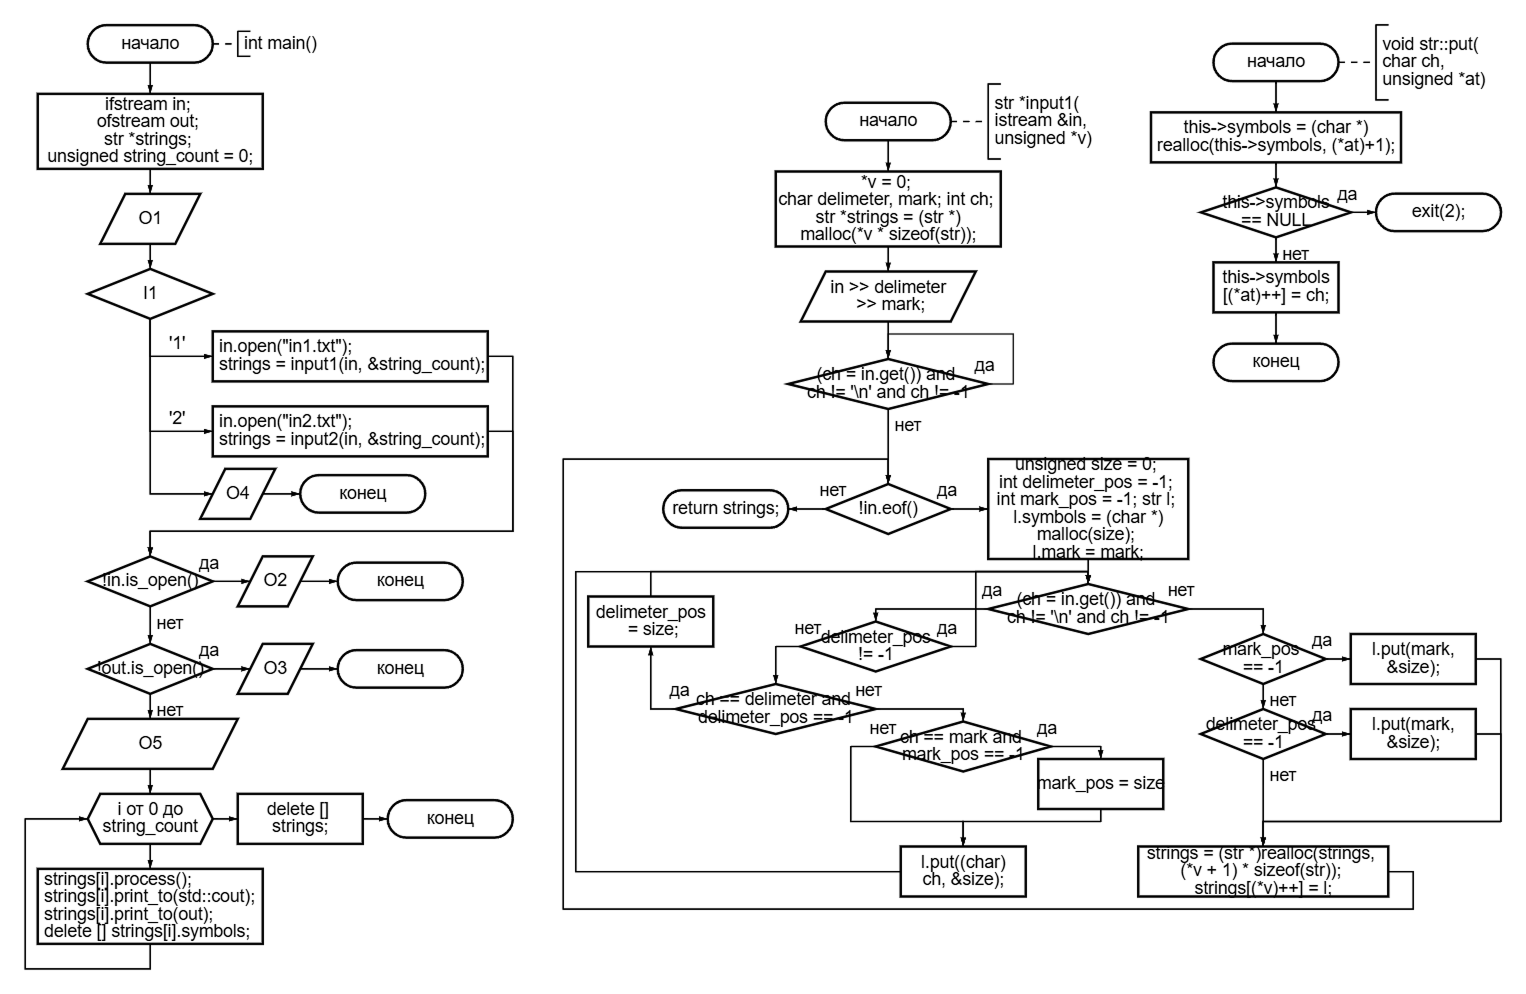
\includegraphics[width=0.9\linewidth]{figures/lab1/Frame 3.png}
    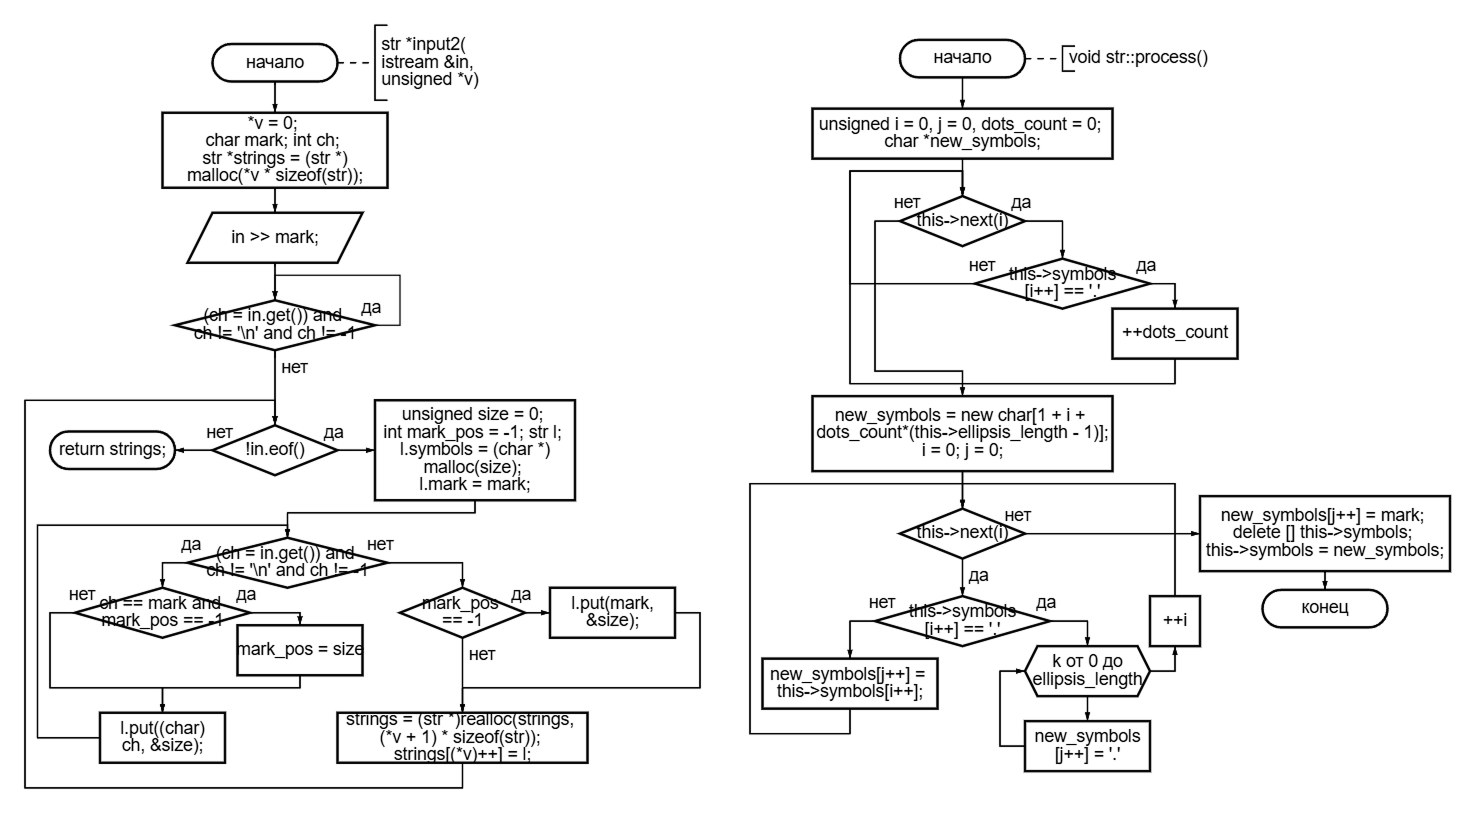
\includegraphics[width=0.9\linewidth]{figures/lab1/Frame 4.png}
\end{figure}

\section{Исходный код программы}
{\ttfamily\scriptsize
\begin{verbatim}
// Преобразовать заданную строку следующим образом: каждую точку заменить многоточием
// Даричев Егор, а.г. 4352

#include <fstream>
#include <iostream>
#include <cmath>
#include <iomanip>

using std::istream, std::ifstream, std::ofstream, std::ostream;
using std::noskipws;
using std::endl;


struct str {
    char *symbols;
    char mark;

    unsigned ellipsis_length = 3;

    bool next(unsigned i) {
        return this->symbols[i] != this->mark;
    }

    void process() {
        unsigned i = 0, j = 0, dots_count = 0;
        char *new_symbols;

        while (this->next(i)) if (this->symbols[i++] == '.') ++dots_count;
        new_symbols = new char[1 + i + dots_count*(this->ellipsis_length - 1)];
        i = 0; j = 0;

        while (this->next(i)) {
            if (this->symbols[i] == '.') {
                for (unsigned k = 0; k < this->ellipsis_length; ++k) new_symbols[j++] = '.';
                ++i;
            } else new_symbols[j++] = this->symbols[i++];
        }

        new_symbols[j++] = mark;

        delete [] this->symbols;
        this->symbols = new_symbols;
    }

    void print_to(ostream &out, bool show_mark = true, bool newline = true) {
        unsigned i = 0;
        while (this->next(i)) out << this->symbols[i++];
        if (show_mark) out << this->symbols[i];
        if (newline) out << endl;
    }

    void put(char ch, unsigned *at) {
        this->symbols = (char *)realloc(this->symbols, (*at)+1);
        if (this->symbols == NULL) exit(2);
        this->symbols[(*at)++] = ch;
    }
};

str *input1(istream &in, unsigned *v) {
    *v = 0;
    char delimeter, mark;
    int ch;
    str *strings = (str *)malloc(*v * sizeof(str));

    in >> delimeter >> mark;
    while ((ch = in.get()) and ch != '\n' and ch != -1);

    if (in.eof()) exit(1);

    while (!in.eof()) {
        unsigned size = 0;
        int delimeter_pos = -1;
        int mark_pos = -1;

        str l;
        l.symbols = (char *)malloc(size);
        l.mark = mark;

        while ((ch = in.get()) and ch != '\n' and ch != -1) {
            if (delimeter_pos != -1) continue;
            if (ch == delimeter and delimeter_pos == -1) {
                delimeter_pos = size;
                continue;
            }
            else if (ch == mark and mark_pos == -1) mark_pos = size;

            l.put((char)ch, &size);
        }

        if (mark_pos == -1) l.put(mark, &size);
        else if (delimeter_pos == -1) l.put(mark, &size);

        strings = (str *)realloc(strings, (*v + 1) * sizeof(str));
        if (strings == NULL) exit(3);
        strings[(*v)++] = l;
    }

    std::cout << endl;
    return strings;
}

str *input2(istream &in, unsigned *v) {
    *v = 0;
    char mark;
    int ch;
    str *strings = (str *)malloc(*v * sizeof(str));

    in >> mark;
    while ((ch = in.get()) and ch != '\n' and ch != -1);

    if (in.eof()) {
        exit(1);
    }

    while (!in.eof()) {
        unsigned size = 0;
        int mark_pos = -1;

        str l;
        l.symbols = (char *)malloc(size);
        l.mark = mark;

        while ((ch = in.get()) and ch != '\n' and ch != -1) {
            if (l.symbols == NULL) exit(2);
            if (ch == mark and mark_pos == -1) mark_pos = size;
            l.put((char)ch, &size);
        }

        if (mark_pos == -1) l.put(mark, &size);

        strings = (str *)realloc(strings, (*v + 1) * sizeof(str));
        if (strings == NULL) exit(3);
        strings[(*v)++] = l;
    }

    std::cout << endl;
    return strings;
}


int main() {
    ifstream in;
    ofstream out;
    str *strings;
    unsigned string_count = 0;

    std::cout << "Задание: Преобразовать заданную строку следующим образом:
каждую точку заменить многоточием\n"
              << "Даричев Егор а.г. 4352\n"
              << "Введите номер варианта ввода: ";
    switch (std::cin.get())
    {
    case '1':
        in.open("in1.txt");
        strings = input1(in, &string_count);
        break;
    case '2':
        in.open("in2.txt");
        strings = input2(in, &string_count);
        break;

    default:
        std::cout << "Неверный номер варианта" << endl;
        return 0;
    }

    if (!in.is_open()) {
        std::cout << "Не удалось открыть файл ввода" << endl;
        return 0;
    }

    out.open("out.txt");
    if (!out.is_open()) {
        std::cout << "Не удалось открыть файл вывода" << endl;
        return 0;
    }

    in >> noskipws;

    std::cout << "Вывод результата в консоль и выходной файл:" << endl;
    for (unsigned i = 0; i < string_count; ++i) {
        strings[i].process();
        strings[i].print_to(std::cout);
        strings[i].print_to(out);
        delete [] strings[i].symbols;
    }
    delete [] strings;
}

\end{verbatim}
}

\section{Результаты работы программы}

\begin{xltabular}
    {\linewidth}{|H|H|} \hline
    \multicolumn{1}{|h}{Вход 1} & \multicolumn{1}{|h|}{Вход 2} \\ \hline
{\ttfamily\footnotesize *@

Donec in leo luctus. Viverra ligula tincidunt, molestie neque. Sed quis elit eget risus tempor ornare at quis nunc.

In quis metus auctor... iaculis lorem vel... aliquam nibh!\&\%\&!!! Fusce a risus rhoncus,,,;: ad.

Donec vitae mauris. Non accumsan.

Donec in leo luctus. Viverra.@berla tincros*asdfgedo.

Donec in leo luctus. Viverra.*berla tincros@asdfgedo.

Donec in leo luctus. @@Viverra ligula*** tincidunt, mol@@estie neque. Se@*d quis
} & {\ttfamily\footnotesize @

Donec in leo luctus. Viverra ligula tincidunt, molestie neque. Sed quis elit eget risus tempor ornare at quis nunc.

In quis metus auctor... iaculis lorem vel... aliquam nibh!\&\%\&!!! Fusce a risus rhoncus,,,;: ad.

Donec vitae mauris. Non accumsan.

Donec in leo luctus. Viverra.@berla tincros*asdfgedo.

Donec in leo luctus. Viverra.*berla tincros@asdfgedo.

Donec in leo luctus. @@Viverra ligula*** tincidunt, mol@@estie neque. Se@*d quis
} \\ \hline
    \multicolumn{1}{|h}{Выход 1} & \multicolumn{1}{|h|}{Выход 2} \\ \hline
{\ttfamily\footnotesize
Donec in leo luctus... Viverra ligula tincidunt, molestie neque... Sed quis elit eget risus tempor ornare at quis nunc...@

In quis metus auctor......... iaculis lorem vel......... aliquam nibh!\&\%\&!!! Fusce a risus rhoncus,,,;: ad...@

Donec vitae mauris... Non accumsan...@

@

Donec in leo luctus... Viverra...@

Donec in leo luctus... Viverra...@

Donec in leo luctus... @
} & {\ttfamily\footnotesize
Donec in leo luctus... Viverra ligula tincidunt, molestie neque... Sed quis elit eget risus tempor ornare at quis nunc...@

In quis metus auctor......... iaculis lorem vel......... aliquam nibh!\&\%\&!!! Fusce a risus rhoncus,,,;: ad...@

Donec vitae mauris... Non accumsan...@

@

Donec in leo luctus... Viverra...@

Donec in leo luctus... Viverra...*berla tincros@

Donec in leo luctus... @
} \\ \hline
\end{xltabular}

\section{Вывод о проделанной работе}
В ходе выполнения работы я научился такой структуре данных, как маркированная строка, как работать с ней, распределяя память динамически.

\end{document}
